\documentclass[]{article}
\usepackage[utf8]{inputenc}
\usepackage[english,russian]{babel}
%\usepackage[12pt]{extsizes}
\usepackage{amsmath}
\usepackage{enumerate}

%\usepackage[left=3cm, top=1.5cm, right=1.3cm, bottom=2cm, nohead, footskip=10mm]{geometry}
\usepackage[12pt]{extsizes}
\linespread{1.3}
\usepackage[left=3cm, top=1.5cm, right=1.3cm, bottom=2cm, nohead, footskip=10mm]{geometry}


\usepackage[absolute,overlay]{textpos}
\usepackage{indentfirst}
\usepackage{float}
\restylefloat{table}
\usepackage{hyperref}
\usepackage{mathtext}
\usepackage{amsfonts}
\usepackage{amsthm}
\usepackage{tikz}
\usepackage{xspace}
\usetikzlibrary{shapes,positioning,shadows,trees,automata,arrows.meta,shapes.geometric}
\usepackage{pgf-pie}
\usepackage{chngcntr}
\usepackage{pdfpages}
\usepackage{systeme}
\usepackage{empheq}
\numberwithin{equation}{section}
\usepackage{caption}
\DeclareCaptionLabelSeparator{none}{. }
\captionsetup{labelsep=none}


\pagestyle{plain}

\renewcommand{\labelenumii}{\theenumii}
\renewcommand{\theenumii}{\arabic{enumii}.}

\begin{document}
    \thispagestyle{empty}
	\begin{center}
		Министерство образования и науки Российской Федерации\\
		Санкт-Петербургский государственный технический университет\\
		Институт прикладной математики и механики\\
		Кафедра <<Телематика>>\\
		\vspace{5cm}
		\textbf{\textbf{ЛАБОРАТОРНАЯ РАБОТА}}\\
        \vspace{0.5cm}
        \textbf{ПО ТЕМЕ}\\
        \vspace{0.5cm}
		\textbf{\textbf{<<Алгоритмы композиции>>}}\\
		\vspace{3cm}
		по направлению 02.04.01.02 <<Организация и управление суперкомпьютерными системами>>
	\end{center}
	\vspace{2cm}
	\begin{tabular} {l l l}
	\hspace{9.5cm} & Выполнил: & \\
	& Студент гр. 13643.1 & Титов А.И.\\
	& Проверил: & Уткин Л.В.
	\end{tabular}
	\vspace{4.5cm}
	\begin{center}
		Санкт-Петербург\\
		2019
    \end{center}


	\renewcommand\contentsname{Оглавление}
	\tableofcontents

    \newpage
    \section*{Постановка задачи}
    \addcontentsline{toc}{section}{Постановка задачи}

    \begin{enumerate}
        \item Исследовать зависимость тестовой ошибки от количества деревьев в ансамбле для алгоритма adaboost.M1 на наборе данных Vehicle из пакета mlbench (обучающая выборка должна состоять из 7/10 всех прецедентов, содержащихся в данном наборе данных). Построить график зависимости тестовой ошибки при числе деревьев, равном 1, 11, 21, . . . , 301, объясните полученные результаты.
        \item Исследовать зависимость тестовой ошибки от количества деревьев в ансамбле для алгоритма bagging на наборе данных Glass из пакета mlbench (обучающая выборка должна состоять из 7/10 всех прецедентов, содержащихся в данном наборе данных). Построить график зависимости тестовой ошибки при числе деревьев, равном 1, 11, 21, . . . , 201, объясните полученные результаты.
        \item Реализовать бустинг алгоритм с классификатором K ближайших соседей. Сравнить тестовую ошибку, полученную с использованием данного классификатора на наборах данных Vehicle и Glass, c тестовой ошибкой, полученной с использованием единичного дерева классификации.
    \end{enumerate}

    \newpage
    \section{Набор данных <<Vehicle>>}
    Был построен классификатор на основе алгоритма бустинга adaboost. Алгоритм был предложен Йоавом Фройндом и Робертом Шапире в 1996ом году. Алгоритм использует дерево решений в качестве классификатора. Был построен график ошибки в зависимости от количества использованных слоев классификаторов (рис. 1). Было установлено, что минимальная ошибка достигается при количестве деревьев: 31, 61, 111.
    \begin{figure}[H]
        \centering
        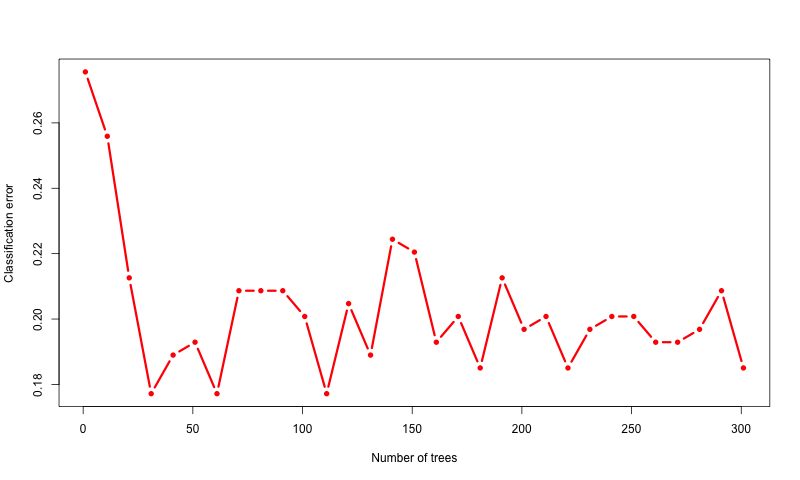
\includegraphics[width = 0.9\linewidth]{data/Vehicle_num_trees.png}
        \caption{Зависимость ошибки от количества использованных деревьев для набора <<Vehicle>>}
    \end{figure}

    \section{Набор данных <<Glass>>}
    Был построен классификатор на основе алгоритма bagging (bootstrap bagging). Алгоритм был предложен Лео Брейманом в 1994ом году. Алгоритм также использует дерево решений в качестве классификатора, но подход использования иной в сравнении с adaboost. Был построен график ошибки в зависимости от количества использованных слоев классификаторов (рис. 2). Было установлено, что минимальная ошибка достигается при количестве деревьев: 41, 81, 101, 131, 141, 151, 161, 191.
    \begin{figure}[H]
        \centering
        \includegraphics[width = 0.9\linewidth]{data/Glass_num_trees.png}
        \caption{Зависимость ошибки от количества использованных деревьев для набора <<Glass>>}
    \end{figure}

    \section{Использование KNN в алгоритме бустинга}

    Задание ясно, но труднореализуемо по причине отсутствия готовых решений в библиотеках, таких как были в предыдущих заданиях (<<adaboost>> и <<bagging>>). Существует реализация с помощью инструментария библиотеки <<caret>>, но такое решение слишком ручное, поэтому очень трудозатратно и потребует много времени для реализации. Поэтому в рамках выполнения лабораторной работы были изучены вырианты реализации задания, но само задание выполнено не было. Ко всему прочему - требуемый вывод был все же сделан. Применение расширенного с помощью бустинга алгоритма knn может привести к повышению точности результатов, но не всегда это имеет смысл, так как сам по себе подход последовательного ансамбля может оказаться весьма ресурсозатратным и дать не достаточный прирост точности, а в некоторых случаях даже проиграть по точности перед применением более простых методов.

\end{document}
